% siminos/xiong/thesis/chapters/dissipative.tex
% $Author: xiong $ $Date: 2017-03-31 22:38:06 -0400 (Fri, 31 Mar 2017) $


%% ======================================================================
\section{Dissipative nonlinear systems}
\label{sect:diss}

Dissipative nonlinear systems described by PDEs
are infinite\dmn\ in principle, but a lot of them
exhibit finite dimensional behavior after a
transient period of evolution. In this context,
the concept of global attractor was
introduced to describe the asymptotic behavior of a dissipative
system. Different definitions of dimension
have been proposed to characterize the dimensionality of a
global attractor. The estimated dimension provides a sense
of the
size of the global attractor, but such numbers, usually not integers,
are smaller than the number
of degrees of
freedom needed to determine the system. This is where the inertial
manifold is introduced to account for the question that how many modes
are needed to effectively describe a dissipative chaotic system.

\subsection{Global attractor}

Before we introduce a global attractor, let us define all necessary
tools first. Here we follow expositions of
Robinson\rf{Robinson2001} and Temam\rf{infdymnon}.
Let a dynamical system $\ssp(t)$, $t\ge 0$
be defined in a \statesp\ $\pS$. $\pS$ is a Hilbert space, usually
the $L^2$ space, with $L^2$ norm the appropriate norm for measuring
distances between different states.
$\semiflow{t}$ is a \emph{semigroup} that
evolves the system forward in time, $\ssp(t) = \semiflow{t}\ssp_0$, with following
properties:
\begin{align*}
  & \semiflow{0} = 1 \,, \\
  & \semiflow{t}\semiflow{s} = \semiflow{s+t} \,, \\
  & \semiflow{t}\ssp_0 \; \text{is continuous in} \; \ssp_0\; \text{and}\; t
    \,.
\end{align*}
An absorbing set is a bounded set that attracts all orbits in this
system. We define dissipative systems as follows.
\begin{definition}
  A semigroup is dissipative if it possesses a compact
  absorbing set $B$ and for any bounded set $X$ there exists
  a $t_0(X)$ such that
  \[
    \semiflow{t}X \subset B\quad \text{for all} \quad t \ge t_0(X)
  \]
  \label{def:dissi}
\end{definition}
% \advise{I don't think this is accurate. What if the absorbing set is a
% single point? Then this definition makes no sense. $\semiflow{t}X$ should be in,
% or equal, to B. Or you have to require that B is an open set.}
% \Xiong{I think I did not mention that $\subset$ only means a subset not a proper
% subset $\subsetneq$. I follow the convention in\rf{Robinson2001}. I add one more
% sentence below to emphasize it.
% }
Here, symbol $\subset$ means that the left side is a proper subset of, or equal to
the right side.
Therefore,  in a dissipative system,
all trajectories eventually enter and stay in
an absorbing set. Moreover, we say that
a set $X\subset \pS$ is \emph{invariant} if
\begin{equation}
  \label{eq:invariant}
  \semiflow{t}X = X  \quad \text{for all} \quad t \ge 0
\end{equation}
and a set $X\subset \pS$ is \emph{positive-invariant} if
\begin{equation}
  \label{eq:pos_invar}
  \semiflow{t}X \subset X  \quad \text{for all} \quad t \ge 0
  \,.
\end{equation}
With the above setup, let us turn to the definition of a global
attractor.
\begin{definition}
  The global attractor $\mathcal{A}$ is
  the maximal compact invariant set
  \begin{equation}
    \semiflow{t}\mathcal{A} = \mathcal{A} \quad \text{for all} \quad
    t \ge 0
    \label{eq:ga1}
  \end{equation}
  and the minimal set that attracts all bounded sets:
  \begin{equation}
    \dist(\semiflow{t}X, A) \to 0 \quad \text{as} \quad t\to\infty
    \label{eq:ga2}
  \end{equation}
  for any bounded set $X\subset \pS$, where $\pS$ is the \statesp.
\end{definition}
Here, the distance between two sets is defined as
\begin{equation}
  \label{eq:dist}
  \dist(X, Y) = \sup_{x\in X} \inf_{y\in Y} |x - y|
  \,.
\end{equation}
Requirement \refeq{eq:ga1} says that
a global attractor does not contain any transient trajectories,
and any trajectory in the \statesp\ will approach the
global attractor arbitrarily close according to \refeq{eq:ga2}.
Note,
the definition emphasizes that the attractor is ``global/maximal'' because
it attracts any bounded sets in \statesp\ $\pS$. If it only attracts some
portion of $\pS$, then it is an
attractor but not a global one. On the other hand,
the word ``minimal'' in the definition
is a consequence of \refeq{eq:ga2}. Suppose there is a
smaller compact set $\mathcal{B}\subsetneq \mathcal{A}$, then
we take the bounded set $X = \mathcal{A}$ and get
$\dist(\semiflow{t}\mathcal{A}, \mathcal{B}) = \dist(\mathcal{A}, \mathcal{B})$
which cannot reach zero in a Hausdorff space.
\footnote{
  A Hausdorff space is a topological space in which distinct points
  have disjoint neighborhoods. Therefore, distinct points have
  positive distance.
}

Now, we turn to the question that whether a global attractor exists
for a dissipative system, and
if it does, then what subsets in the \statesp\
should be included in it. We have
some expectations in mind. First,
the concept of global attractor was introduced to assist the
study of the asymptotic behavior in a
dissipative system, so we expect its existence in
dissipative systems.
Second, the global attractor should include all the important
dynamical structures of a dissipative system, such as equilibria,
\po s, their unstable manifolds, homoclinic/heteroclinic
orbits and so on. If a global attractor fails either of these
two requirements, then it makes no sense to use it in practice.
Both questions are answered by the following theorem.
\begin{theorem}
  If $\semiflow{t}$ is dissipative and $B\subset \pS$ is a compact absorbing
  set then there exists a global attractor $\mathcal{A} = \omega(B)$.
  \label{them:attractor}
\end{theorem}
Here, $\omega(B)$ is the $\omega$-limit set of $B$. For any
subset $X\subset \pS$, its $\omega$-limit set is defined as
\begin{equation}
  \label{eq:omega}
  \omega(X) = \{y :
  \text{there exist sequences}\; t_n\to\infty\;\text{and}\; \ssp_n\in X \;
  \text{with}\; \semiflow{t_n}\ssp_n\to y\}
  \,.
\end{equation}
An equivalent limit supremum definition is
\[
  \omega(X) = \bigcap_{t\ge 0}\overline{\bigcup_{s\ge t}\semiflow{s}X}
\]
Here, the overbar of a set means taking the closure of this set.
It is easy to see
that the $\omega$-limit set of a single point $\ssp$ consists
of all limiting points of $\semiflow{t_n}\ssp$
given it converges for a sequence of $\{t_n\}_{n=1}^\infty$,
$t_n\to\infty$,
i.e.,
\begin{equation}
  \omega(\ssp) = \{y :
  \text{there exists a sequence}\; t_n\to\infty \;
  \text{with}\; \semiflow{t_n}\ssp \to y
  \}
  \,.
  \label{eq:omega2}
\end{equation}
Theorem \ref{them:attractor} not only claims the existence of a
global attractor in a dissipative system but also
gives the explicit form of it as the $\omega$-limit set of a bounded
set. Now, let us check whether $\omega(B)$ contains all the important
invariant structures in this system as expected.
By definition \refeq{eq:omega} and \refeq{eq:omega2}, we can obtain
the $\omega$-limit set for a few invariant
dynamical structures.
For an equilibrium $\ssp$: $\semiflow{t}\ssp=\ssp$, so
$\omega(\ssp) = \ssp$.
For a \po\ $p$, $\omega(p) = p$,
and for any $\ssp\in p$, $\omega(\ssp) = p$.
These two simple examples may tempt you to
think that $\cup_{\ssp\in X}\omega(\ssp) = \omega(X)$. However, this
is not true. Actually, what we only know is that
\begin{equation}
  \label{eq:omega3}
  \bigcup_{\ssp\in X}\omega(\ssp)\subset \omega(X)
  \,.
\end{equation}
Usually, the left-side set in \refeq{eq:omega3} is much smaller than
the right-side set. To illustrate this point,
\reffig{fig:attractor_portrait}, taken from\rf{Robinson2001}, depicts a planar system
with 3 equilibria $\{a, b, c\}$. $a$ and $c$ are stable.
$b$ has a homoclinic orbit denoted as $W^u(b)$
\footnote{
  The stable and unstable manifolds of a subset $X\subset \pS$ are denoted respectively
  as $W^s(X)$ and $W^u(X)$.
}
since it is
also an unstable manifold of $b$. For any $\ssp\in W^u(b)$,
$\omega(\ssp) = b$. However, for the whole orbit
$\omega(W^u(b)) = W^u(b)$. An intuitive explanation goes as follows.
For any $y\in W^u(b)$ and a $t_n > 0$, we can find a point $\ssp_n$
ahead of $y$ on the homoclinic orbit $\ssp_n\in W^u(b)$
such that $\semiflow{t_n}\ssp_n = y$. The larger $t_n$ is, the closer $\ssp_n$ is to $b$.
It takes an infinitely long time to go backward from $y$ to $b$.
So we find sequences $t_n\to \infty$ and $\ssp_n \in W^u(b)$ such that
$\semiflow{t_n}x_n \to y$, and by definition, $y\in \omega(W^u(b))$.
The same argument can be applied
to the bounded stable manifold of $c$ in \reffig{fig:attractor_portrait}(a),
$\omega(W^s(c)) = W^s(c)$.
\begin{figure}[h]
  \centering
  (a)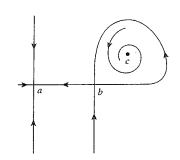
\includegraphics[width=0.4\textwidth]{attractor_portrait_2dsystem}
  (b)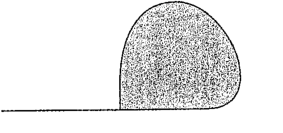
\includegraphics[width=0.5\textwidth]{attractor_2dsystem}
  \caption[The global attractor of a 2d system]{
    (a) \Statesp\ portrait of a 2d system.
    (b) The corresponding global attractor.
  }
  \label{fig:attractor_portrait}
\end{figure}

The $\omega$-limit sets of equilibria, \po s, and homoclinic
orbits are the objects
themselves, so they all belong to the global attractor,
as we would expect. Meanwhile, concerning the stable and unstable manifolds,
we have the following theorem.
\begin{theorem}
  The unstable manifolds and bounded stable manifolds
  of a compact invariant set are contained in the global attractor.
  \label{them:unstable}
\end{theorem}
We stress that the global attractor does not contain unbounded
stable/unstable manifolds. Unstable manifolds are intrinsically bounded
in dissipative systems,
so we omit the word ``bounded'' in front of it in theorem
\ref{them:unstable}. The explanation is simple.
Let $\ssp(t)$  be a point in the unstable manifold of an invariant set $X$, \ie,
$\ssp(t) \in W^{u}(X)$, then $\ssp(t)$ approaches $X$ for $t\to -\infty$ by
definition,
and $\ssp(t) \in B$ when $t\to\infty$ because the system is dissipative with
$B$ an absorbing set. Therefore, unstable manifold $W^u(X)$ is bounded.
However, not all stable manifolds are bounded. For example, one\dmn\
dissipative system $\dot{\ssp} = -\lambda \ssp$, $\lambda>0$
has a global attractor $\ssp=0$, but its stable manifold
extends to $\ssp\to\pm\infty$.
Such a distinction between stable and unstable
manifolds in dissipative systems is crucial for us to understand the finite
dimensionality of such systems.
In an infinite\dmn\ system described by a PDE, an unstable
invariant structure usually has only a few unstable modes and
the rest, infinite many, are all stable modes. Only a finite
subset of these stable modes participates in the dynamics.
As we shall show in this thesis,
the rest stable modes are
decoupled from other modes, decay exponentially, and do not belong to
the global attractor.

In the example shown in \reffig{fig:attractor_portrait}(a),
the 3 equilibria $\{a, b, c\}$, the
stable manifold of $c$, the homoclinic orbit of $b$ and the
heteroclinic orbit from $b$ to $a$ compose the global attractor,
which is shown in \reffig{fig:attractor_portrait}(b).


\paragraph{The global attractor in the Lorenz system}
We now prove the existence of a global attractor for the Lorenz system
to illustrate the concepts introduced in this section.
Theorem \ref{them:attractor} tells us that the key point of showing the
existence of a global attractor is to find a compact absorbing set $B$
in the system. For Lorenz system
\begin{align*}
  \dot{x} & = -\sigma x + \sigma y \\
  \dot{y} & = rx - y - xz \\
  \dot{z} & = xy - bz
\end{align*}
with $\sigma, r, b > 0$, consider
\[
  V(x, y, z) = x^2 + y^2 + (z-r-\sigma)^2
  \,.
\]
Then,
\begin{align*}
  \frac{dV}{dt}
  & = -2\sigma x^2 - 2y^2 - 2bz^2 + 2b(r+\sigma)z \\
  & = -2\sigma x^2 - 2y^2 - b(z-r-\sigma)^2 -bz^2 + b(r+\sigma)^2 \\
  & \le -\alpha V + b(r+\sigma)^2
\end{align*}
Here $\alpha = \min(2\sigma, 2, b)$.
By the Gronwall inequality, we obtain
\[
  V \le \frac{2b(r+\sigma)^2}{\alpha}
  \,.
\]
\begin{lemma}
  (Gronwall's Inequality) If
  \[
    \frac{du}{dt} \le au+b
    \,,
  \]
  then
  \[
    \ssp(t) \le (\ssp_0 + \frac{b}{a})e^{at} - \frac{b}{a}
    \,.
  \]
  \label{lem:Gronwall}
\end{lemma}
Therefore, there is an absorbing sphere
$S$ with radius $(2b/\alpha)^{1/2}(r+\sigma)$ in Lorenz system.
So a global attractor exists and it is given as $\omega(S)$.

\subsection{The dimension of an attractor}

Though the \statesp\ $\pS$ may be infinite\dmn,
after a transient period of evolution,
the dynamics is usually
determined only by a finite number of degrees of freedom.
The global attractor lives in a finite\dmn\ subspace of the
\statesp. Consequently, the study of the dimension of the global
attractor is crucial for us to understand the longtime behavior of
this system.
According to \refref{FaOttYo83}, the types of dimensions of chaotic attractors
can be classified into three categories. One is \emph{fractal dimensions},
based purely on the
geometry of the attractor such as the
box-counting dimension $D_{C}$ and the Hausdorff dimension $D_H$.
The second type
incorporates the frequency with which a typical
trajectory visits various parts of the attractor, namely the natural
measure of the attractor, such as  the information dimension $D_I$,
correlation
dimension $D_\mu$\rf{GraPro83a}, and so on. The third one,
Kaplan-Yorke
dimension $D_{KY}$ is defined in terms of the dynamical properties of an
attractor rather than the geometry or the natural measure.
Kaplan and Yorke\rf{KapYor79a, FKYY83}
initially conjectured that $D_{KY} = D_{C}$, but later
it was shown that $D_{KY}$ is an upper bound of the information dimension.
Some comparison of these various definitions of dimension can be found in
\refrefs{FaOttYo83, GraPro83a,Hunt96}. In this subsection, we list some
representative definitions related to our research.

\paragraph{Box-counting dimension (capacity dimension, Kolmogorov dimension)}
By using a minimal set of balls with radius $\epsilon$ to cover the
attractor and record the number of balls $N(\epsilon)$,
the \emph{box-counting dimension}
is given by
\begin{equation}
  \label{eq:dc}
  D_C = \limsup_{\epsilon \to 0} \frac{\log N(\epsilon)}{\log(1/\epsilon)}
\end{equation}
Note, we can also use cubes of side length $\epsilon$, which
does not change the result.
Basically, $D_C$ tells us how dense the state points are inside the
attractor. Trivial cases, like $D_C = 1$ for a straight line and
$D_C = 2$ for an area, are within our expectation, but for
fractal objects, it usually produces fraction/irrational numbers.
For instance, $D_C = \log 3/ \log 2$ for the Sierpinski triangle shown in
\reffig{fig:sier-tri}.
\begin{figure}[h]
  \centering
  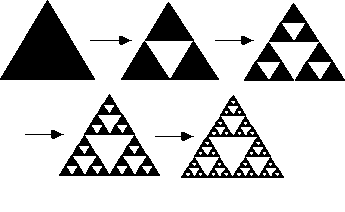
\includegraphics[width=0.5\textwidth]{sierp-det}
  \caption[The Sierpinski triangle]{
    The iterative process to get the Sierpinski triangle
    (from \refref{Devaney95}).
  }
  \label{fig:sier-tri}
\end{figure}


\paragraph{Hausdorff dimension}
The box-counting dimension uses balls of the same radius $\epsilon$
to cover the
attractor. Here, we try to cover the attractor with nonuniform open balls
whose radius is no larger than $\epsilon$.
First, we define the  $d$\dmn\ Hausdorff measure of a set $X$ in
$\pS$.
\begin{equation}
  \label{eq:haus_measure}
  \mathcal{H}^d(X) = \liminf_{\epsilon\to 0} \left\{\sum_{i=0}^\infty r_i^d :
    r_i < \epsilon \text{ and }
    X \subset \bigcup_{i=0}^\infty B_{r_i}(\ssp_i)
  \right\}
  \,.
\end{equation}
Here, $B_{r_i}(\ssp_i)$ is a $d$\dmn\
open ball centered at $\ssp_i$ with radius $r_i$. The definition
is analogous to the definition of Lebesgue measure. The basic idea is to estimate the
volume of the attractor by the total volume of finer and finer countable
$d$\dmn\ covering balls, where $d$ is a parameter in this measure. If $d$ is
larger than the actual dimension of the attractor, then $\mathcal{H}^d(X) = 0$.
For example, we need $1/2r$ circles whose radius is $r$
to cover a unit one\dmn\ segment. The total
area of these circles goes to zero when $r\to 0$. On the other hand, if $d$ is smaller
than the actual dimension, then $\mathcal{H}^d(X) \to \infty$. For instance, we need
infinitely long one\dmn\ segments to cover a two\dmn\ plane.
Based on this observation,
the \emph{Hausdorff dimension} of a compact set $X$ is defined as
\begin{equation}
  \label{eq:haus}
  D_H(X) = \inf \left\{d : \mathcal{H}^d(X) = 0 \text{ with } d > 0 \right\}
  \,.
\end{equation}
In general, the
Hausdorff dimension is not easy to get for a dynamical system.
But we do have an upper bound
\begin{equation}
  \label{eq:dhlsdc}
  D_H(X) \le D_C(X) \,.
\end{equation}
This relation is easy to understand. In defining Hausdorff dimension we have more
choices of the covering balls than that in box-counting dimension. Also,
\refeq{eq:haus_measure} is taking an infimum of all choices while $D_C$ takes the
supremum. For a rigorous proof of \refeq{eq:dhlsdc}, see \refref{Robinson2001}.

\paragraph{Information dimension}
The fractal dimension does not count the frequency with which each small region
is visited on the attractor. In order to incorporate such information,
the number of covering balls $N(\epsilon)$ is replaced by the entropy
function $-\sum^{N(\epsilon)} P_i \log P_i$, where $P_{i}$ is the probability
contained in cube $c_i$, namely the natural measure $\mu(c_i)$
of the attractor. The information dimension is then given as\rf{FaOttYo83}
\begin{equation}
  \label{eq:di}
  D_I = \lim_{\epsilon \to 0} \frac{-\displaystyle \sum^{N(\epsilon)}_{i=1}
    P_{i} \log P_i}{\log(1/\epsilon)}
  \,.
\end{equation}
The information dimension is no larger than the box-counting dimension, and
$D_I = D_C$ when the natural measure is constant across the attractor.

\paragraph{Kaplan-Yorke dimension (Lyapunov dimension)}
Kaplan and Yorke first proposed the idea of defining the dimension of a
chaotic attractor by the Lyapunov exponents
    \footnote{Actually, they used the magnitudes of
    multipliers or the `Lyapunov numbers', defined as the exponentials of
    the Lyapunov exponents. }
in \refref{KapYor79a}, and later they elaborated their proposal it in \refref{FKYY83}.
Here I sketch their basic idea\rf{RusHanOtt1980}.

Let $\lambda_1 \ge \cdots \ge \lambda_n$
are the Lyapunov spectrum
of an $n$\dmn\ chaotic system ($\lambda_1 > 0$). We try to
determine how many cubes needed to cover the neighborhood of a template
point $\ssp(0)$ as the system evolves. Suppose the neighborhood is an
$n$\dmn\ parallelogram with initially each edge oriented in the covariant
direction at $\ssp(0)$, and the number of $\epsilon$-cubes needed
to cover this parallelogram is $N(\epsilon)$; then after an infinitesimal
time $\delta t$, the neighborhood moves to $\ssp(\delta t)$ and the parallelogram
gets stretched/contracted in each covariant direction.
Choose some $j+1$ such that
$\lambda_{j+1} < 0$, we use a smaller cube with length
$e^{\lambda_{j+1} \delta t}\epsilon$ to cover the new neighborhood, then
\begin{equation}
N(e^{\lambda_{j+1} \delta t}\epsilon) =
\left( \prod_{i=1}^{j} e^{(\lambda_i - \lambda_{j+1})\delta t}\right)
N(\epsilon)
\label{eq:ky_relation}
\end{equation}
Let's explain the coefficient above. The $i$th direction with $i<j+1$
has been stretched by a factor $e^{\lambda_i \delta t}$, and the
new cube length is $e^{\lambda_{j+1} \delta t}\epsilon$, so it needs
$e^{(\lambda_i - \lambda_{j+1})\delta t}$ times more cubes along this direction.
Also, since choose $\lambda_{j+1} < 0$, then for the $i$th direction
with $i > j+1$, the original number of cubes along this direction
is enough to cover it, which means the above formula is actually
over-counting in this direction. The exponential law
$N(\epsilon) \propto \epsilon^{-d}$ from \refeq{eq:dc} is valid
when $\epsilon$ is small enough. Then \eqref{eq:ky_relation} reduces to
$(e^{\lambda_{j+1} \delta t}\epsilon)^{-d}  =
\prod_{i=1}^{j} e^{(\lambda_i - \lambda_{j+1})\delta t} \epsilon^{-d}$ and thus
\begin{equation}
  d(j) = j - \frac{\sum_{i=1}^{j} \lambda_i}{\lambda_{j+1}}
  \,.
  \label{eq:ky1}
\end{equation}
Just as stated above, formula \refeq{eq:ky1} is an upper bound of the dimension.
We need to find the smallest $d(j)$ under condition $\lambda_{j+1} < 0$.
\begin{align*}
  d(j+1) - d(j) &= 1 -\frac{\sum_{i=1}^{j+1} \lambda_i}{\lambda_{j+2}}
  + \frac{\sum_{i=1}^{j} \lambda_i}{\lambda_{j+1}} \\
  & = \frac{(\lambda_{j+2} - \lambda_{j+1})(\lambda_1 + \cdots + \lambda_{j+1})}
  {\lambda_{j+2}\lambda_{j+1}}
\end{align*}
Let $\lambda_1 + \cdots + \lambda_k \ge 0$ and
$\lambda_1 + \cdots + \lambda_{k+1} < 0$, then $d_{k+1} > d_{k}$ and
$d_k < d_{k-1}$. Therefore
\begin{equation}
  D_{KY} = k + \frac{\sum_{i=1}^{k} \lambda_i}{|\lambda_{k+1}|}
  \label{eq:ky2}
\end{equation}
with $k$ the largest number making $\lambda_1 + \cdots + \lambda_k$
non-negative.


\paragraph{Summary}
The definitions of dimension introduced in this section provide valuable
information about the size of the global attractor. However,
except for the Kaplan-Yorke dimension, all the other definitions
try to cover the global attractor with cubes statically. The information
about the topological structure of a global attractor has not been
used. On the other hand, strange attractors are almost always
fractal, and thus the dimension is an irrational number.
With this number, we
still do not know how many degrees of freedom are
needed to effectively describe the dynamics of a dissipative PDE in an
infinite\dmn\ space. In the next section, we introduce the concept of the
\emph{inertial manifold} that contains the global attractor and determines
the dynamics by a finite number of degrees of freedom.


\subsection{Inertial manifold}
\label{subsec:IM}

For dissipative chaotic systems, asymptotic orbits are contained in a
lower\dmn\ subspace of
the \statesp\ $\pS$. Thus the effective dynamics can be described by a
finite number of degrees of freedom.
A global attractor usually has fractal dimension, which make it hard to
analyze, so we need to construct
a `tight' smooth manifold that encloses it, and whose dimension gives the
effective degrees of freedom of this system. This
is called the \emph{inertial manifold}\rf{Foias1988a,
Robinson1995, infdymnon, Robinson2001}.

Here we use the concept of
``\emph{slaving}'' in order to understand how the transition from infinite\dmn\
space to finite\dmn\ subspace happens. Let $\ssp(t)$ be a dynamical
system in an infinite\dmn\ \statesp\ $\pS$ governed by
\begin{equation}
  \label{eq:proto}
  \frac{d\ssp}{dt} + \vlo \ssp + \vno(\ssp) = 0
  \,.
\end{equation}
We split the ``velocity'' field into a linear part and a nonlinear part.
Linear
operator $\vlo$ is usually a negative Laplace operator or a higher-order spatial
derivative. If the nonlinear term $\vno(\ssp)$ is weak, then the dynamics is
largely determined by the eigenspaces of $\vlo$. That is why in practice
solution $\ssp(t)$ is usually expanded in terms of the eigenvectors of $\vlo$.
Specifically, if $\vlo$ is a negative Laplace operator, and the system is
defined either on an infinite or periodic domain,
then its eigenvectors are pure Fourier modes.
$\ssp(t)$ is determined by an infinite number of its
Fourier coefficients. We say that \highmode s are \emph{slaved to}
\lowmode s if
there is a map that uniquely maps \lowmode s to \highmode s. With such a map,
the dynamics of the system is totally determined by the \lowmode s. To make this
idea more precise,
let $P_n$ denote the projection from \statesp\ $\pS$ to the subspace spanned
by the eigenvectors of $\vlo$ corresponding to its smallest $n$ eigenvalues,
and let $Q_n = I - P_n$. Ranges of $P_n$ and $Q_n$ are denoted
as $P_n\pS$ and $Q_n\pS$ respectively.
Subspaces $P_n\pS$ and $Q_n\pS$ contain the low and \highmode s of
the solution $\ssp(t)$.
Though $Q_n\pS$ is infinite\dmn\, the effective dynamics is trapped in a
finite\dmn\ subspace of $\pS$. So we anticipate that there is
a map $\Phi:P_n\pS\mapsto Q_n\pS$ that determines the \highmode s
of $\ssp(t)$ given its \lowmode s.
Denote
\begin{equation}
  \label{eq:pq}
  p(t) = P_n\ssp(t) \,,\quad q(t) = Q_n\ssp(t)
\end{equation}
and project \eqref{eq:proto} onto $P_n\pS$, we obtain
\begin{equation}
  \label{eq:projected}
  \frac{dp}{dt} + \vlo p + P_n \vno(p+\Phi(p)) = 0
  \,.
\end{equation}
So we have reduced the dynamics to a
subspace given the existence of such a mapping $\Phi$.
Equation \eqref{eq:projected} is
called the \emph{inertial form} of this system.
The graph of $\Phi$
\[
  \mathcal{G}[\Phi] := \{\ssp: \ssp = p + \Phi(p)\,, p\in P_n\pS\}
\]
defines an $n$\dmn\ manifold $\IM$. This manifold is
proved\rf{Robinson2001} to be an inertial manifold
defined below.
\begin{definition}
  An inertial manifold $\IM$ is a finite\dmn\ Lipschitz manifold,
  which is positively invariant and attracts all trajectories exponentially,
  \begin{equation}
    \label{eq:im_def}
    \dist(\semiflow{t}\ssp_0, \IM) \le C(|\ssp_0|)e^{-kt}\quad
    \text{for some } k > 0 \text{ and all } \ssp_0 \in \pS
    \,.
  \end{equation}
\end{definition}
Lipschitz means $|\Phi(p_1) - \Phi(p_2)| \le L |p_1 - p_2|$ for any
$p_1, p_2\in P_n\pS$ and some positive
constant $L$. The Lipschitz condition
is required for the initial form \refeq{eq:projected} to
have unique solutions.
There are several differences between a global attractor and an inertial manifold.
First, an inertial manifold, by definition, has an integer number of dimensions, but
a global attractor of a chaotic system usually has a fractal dimension.
Second, an inertial manifold is
only positive-invariant \refeq{eq:pos_invar}, but a global attractor is the maximal
invariant subset of $\pS$. Therefore, the global attractor is contained in the
inertial manifold. Third, a global attractor can attract trajectories arbitrarily slowly
by definition \refeq{eq:ga2}, while an inertial manifold attracts trajectories
exponentially fast.

Equation \refeq{eq:im_def} also implies that the error introduced by
approximating $q(t)$ by $\Phi(p(t)$ decays exponentially with time:
\begin{equation}
  |q(t)-\Phi(p(t))| \le C(|\ssp_0|)e^{-kt}
  \,.
  \label{eq:im_def2}
\end{equation}
The reason is as follows. From the definition of distance of two sets
\refeq{eq:dist} and the fact that
$\ssp(t) = \semiflow{t}\ssp_0 = P_n\ssp + Q_n\ssp$, we have
\[
  \dist(\semiflow{t}\ssp_0, \IM) = \inf_{s\in P_n\pS} \left|(P_n\ssp + Q_n\ssp) -
    (s + \Phi(s))\right|
  \,.
\]
Since projection $P_n$ and $Q_n$ are orthogonal to each other, the above
infimum is reached when $s = P_nu$. Thus we have we
\[
  \dist(\semiflow{t}\ssp_0, \IM) = \left|Q_n\ssp - \Phi(P_n\ssp)) \right| =
  \left|q(t) - \Phi(p(t)) \right|
  \,.
\]
The equivalence between \refeq{eq:im_def} and \refeq{eq:im_def2} confirms that
the idea of \emph{mode slaving} works in a dissipative system given the existence
of an inertial manifold. For any point in the \statesp, we can find an
approximate state on the inertial manifold. These two states share the same \lowmode s
and only differ in their
\highmode s. \Highmode s are slaved to \lowmode s,
and their difference decays exponentially. So after a short transient
period, all orbits are effectively captured by the inertial manifold.

An inertial manifold exists in systems which possess the
\emph{strong squeezing property}\rf{Robinson2001}. A system says to have the
strong squeezing property if for any two solutions
$\ssp(t) = p(t) + q(t)$ and $\bar{\ssp}(t) =  \bar{p}(t) + \bar{q}(t)$, the following
two properties hold. (i) the \emph{cone invariance property}: if
\begin{equation}
  \label{eq:ssp1}
  |q(0) - \bar{q}(0)| \le |p(0) - \bar{p}(0)|
\end{equation}
then
\begin{equation}
  \label{eq:ssp2}
  |q(t) - \bar{q}(t)| \le |p(t) - \bar{p}(t)|
\end{equation}
for all $t \le 0$, and (ii) the \emph{decay property}: if
\begin{equation}
  \label{eq:ssp3}
  |q(t) - \bar{q}(t)| \ge |p(t) - \bar{p}(t)|
\end{equation}
then
\begin{equation}
  \label{eq:ssp4}
  |q(t) - \bar{q}(t)| \le |q(0) - \bar{q}(0)| e^{-kt}
\end{equation}
for some $k > 0$. The first property says that initially if two states
satisfy the Lipschitz condition with Lipschitz constant $1$, then
such a Lipschitz condition holds at any later time.
The second property accounts for the exponential attraction \refeq{eq:im_def}
of the inertial manifold.
In practice, it is hard to verify the strong squeezing property
directly. Here we provide an intuitive argument to
show that a large gap in the eigenspectrum of operator $\vlo$ in \refeq{eq:proto}
leads to the strong squeezing property. Let $\vlo$ have eigenvalues
$\lambda_1 \le \lambda_2 \le \cdots$. Inertial form
\refeq{eq:projected} describes the dynamics of the $n$ \lowmode s
which correspond to eigenvalues $\lambda_1,\cdots, \lambda_n$.
The minimal growth rate in subspace $P_n\pS$ is $-\lambda_n$. While, the rest
\highmode s should have approximately the largest growing rate $-\lambda_{n+1}$. If
$-\lambda_{n+1}$ is far smaller than $-\lambda_n$, then we anticipate that
$|p(t)-\bar{p}(t)|$ should grow faster than $|q(t)-\bar{q}(t)|$, so
\refeq{eq:ssp2} holds.
Also, if $-\lambda_{n+1} < 0$, then
\refeq{eq:ssp4} should hold too. Note that we have not taken into consideration the
coupling between low and \highmode s by the nonlinear term
$\vno(\ssp)$ in \refeq{eq:proto}.
Therefore, to ensure strong squeezing property,
the threshold of gap $\lambda_{n+1}-\lambda_{n}$
should depend on $\vno(\ssp)$. Such a \emph{spectral gap condition}
is precisely described in the following theorem.
\begin{theorem}
  \label{them:spectGap}
  If $\vno(\ssp)$ is Lipschitz
  \[
    |\vno(\ssp) - \vno(v)| \le C_1 |\ssp - v|, \quad \ssp, v \in \pS
  \]
  and eigenvalues of $\vlo$ in \refeq{eq:proto} satisfies
  \begin{equation}
    \label{eq:im_gap}
    \lambda_{n+1} - \lambda_n > 4 C_1
  \end{equation}
  for some integer $n$, then the strong squeezing property holds, with
  $k$ in \refeq{eq:ssp4} satisfying $k \ge \lambda_n + 2C_1$.
\end{theorem}
See\rf{Robinson2001} for the proof of this theorem.

The existence of an inertial manifold has been proved
for many chaotic or turbulent systems such as \KSe, \cGLe\ and
the two\dmn\ \NSe\rf{infdymnon}.
Also, numerical methods such as Euler-Galerkin\rf{foias88} and nonlinear
Galerkin method\rf{Marion1989} have been proposed to approximate
inertial manifolds. Approximating
mapping $\Phi:P_n\pS\mapsto Q_n\pS$ requires choosing an appropriate $n$ first.
If $n$ is smaller than the dimension of the inertial manifold, then $\Phi$
fails to describe the inertial manifold. However, if $n$
is far larger than the dimension of the inertial manifold, then simulations on
such approximations to the inertial manifold
are not numerically efficient.
At present, one uses empirical or some test number to truncate the
original system. For example, in\rf{foias88}, 3 modes are
used to represent the inertial manifold of the one\dmn\ \KSe, but this
truncated model is not sufficient to preserve the bifurcation diagram.
At the same time, mathematical upper bounds for the dimension are not always tight.
Therefore, little is known about the exact dimension of inertial manifolds in
dissipative chaotic systems.
